\chapter{Conclusões}
\label{cap:conclusoes}

O Capítulo~\ref{cap:avaliacao} avaliou os quatro componentes. Este reúne o que dessas
medições se retira. Sintetiza o trabalho realizado, apresenta a resposta obtida para cada questão de
investigação, identifica as limitações do estudo e enuncia as linhas de desenvolvimento futuro. Quem o leia fica a saber o que o trabalho estabelece, o que decide sem estabelecer, e o que fica por testar.

\section{Conclusões principais}
\label{sec:con_principais}

O trabalho produziu um sistema em funcionamento e uma avaliação de cada uma das técnicas que o
compõem. O InvestiGator monitoriza doze empresas em ciclo contínuo, entrega alertas explicados a um
canal público e disponibiliza uma página onde ficam registadas tanto as mensagens enviadas como as
decisões que conduziram ao silêncio. Entre 9 de julho e 13 de agosto de 2026 foram entregues
$367$ mensagens, entre 22 de julho e 20 de agosto registaram-se $36\,925$ decisões de triagem,
e a reconstrução da base de precedentes reuniu $38\,214$ casos com impacto medido. Estes números
descrevem um sistema implantado e não uma demonstração construída para o efeito.

A componente que confere ao trabalho o carácter de dissertação não é, contudo, o sistema, mas a
avaliação a que foi submetido. Três das quatro técnicas foram comparadas com alternativas mais
simples, escolhidas e declaradas antes de a medição ser realizada, o que é a condição para que o
resultado possa ser negativo. Numa delas o resultado foi efetivamente negativo. A quarta técnica, a decomposição do movimento, não admite comparação da mesma natureza, uma vez
que a repartição de um retorno não possui referente externo observável. Dela mediu-se o que
permanece falsificável: a qualidade do ajuste que a sustenta, e a capacidade de produzir respostas
distintas para empresas distintas.

A contribuição de engenharia não reside na dimensão do modelo aprendido. O sistema treina um único
modelo, com nove entradas, e esse modelo perde para uma linha de base de uma só variável. A confiança nesse valor, e na conclusão negativa que ele sustenta, depende do que foi preciso
construir em volta dele. A Secção~\ref{sec:sis_ciclo} descreve as sete peças. O conjunto de dados
é rotulado a partir de duas fontes independentes. O rótulo é declarado como decisão, e nove
definições alternativas são medidas em vez de a adotada ser assumida. A separação temporal é verificada por um
procedimento automático. A calibração vem acompanhada da medição e da declaração do enviesamento
que a afeta. Os artefactos ficam sob controlo de versões. O modelo implantado é comprovadamente o
modelo avaliado. E o sistema em funcionamento continua a ser observado. É nesse conjunto, e não no
modelo, que reside o trabalho.

Uma segunda conclusão atravessa os quatro casos de estudo e não pertence a nenhum deles em
particular. Em quatro ocasiões distintas, uma técnica mais simples obteve melhor resultado do que uma
mais sofisticada em condições equivalentes; em três outras sucedeu o inverso, e o sistema conservou
mesmo assim a opção implantada, por uma razão distinta em cada caso. A
Figura~\ref{fig:con_simples} reúne as sete.

\begin{figure}[ht]
\centering
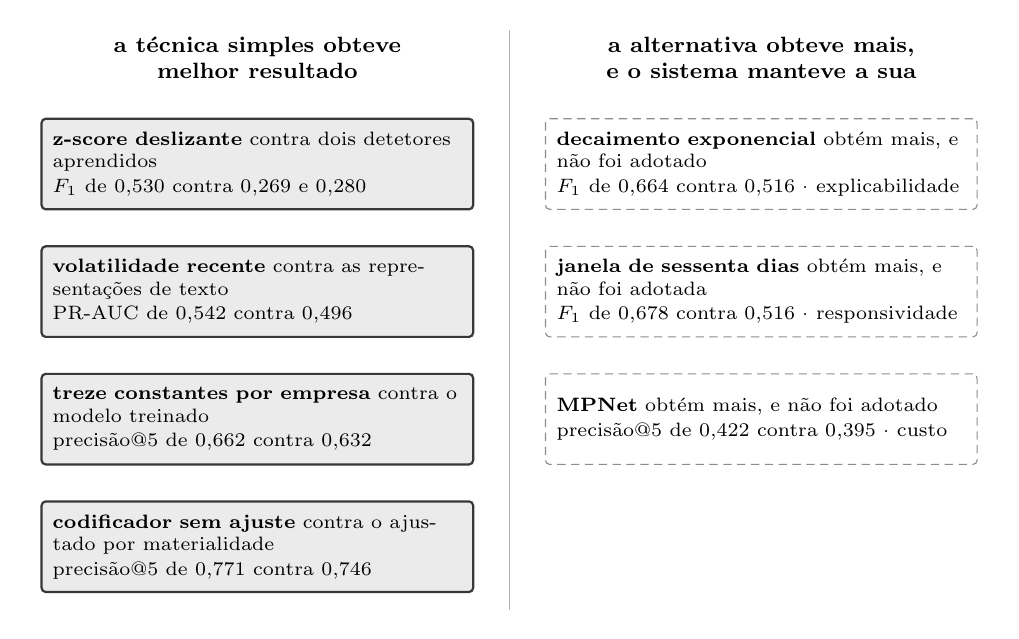
\begin{tikzpicture}[font=\scriptsize,
  cx/.style={draw=black!60, rounded corners=1.5pt, align=left, inner sep=4pt,
        text width=5.2cm, minimum height=1.15cm},
  ganha/.style={cx, fill=black!8, draw=black!78, line width=0.8pt},
  perde/.style={cx, fill=white, draw=black!45, densely dashed},
  cab/.style={font=\footnotesize\bfseries, align=center, text width=5.6cm},
]
  \node[cab] at (0,1.35) {a técnica simples obteve\\melhor resultado};
  \node[cab] at (6.4,1.35) {a alternativa obteve mais,\\e o sistema manteve a sua};
  \node[ganha] at (0,0.0) {\textbf{z-score deslizante} contra dois detetores aprendidos\\[1pt]\scriptsize $F_1$ de $0{,}530$ contra $0{,}269$ e $0{,}280$};
  \node[perde] at (6.4,0.0) {\textbf{decaimento exponencial} obtém mais, e não foi adotado\\[1pt]\scriptsize $F_1$ de $0{,}664$ contra $0{,}516$ · explicabilidade};
  \node[ganha] at (0,-1.62) {\textbf{volatilidade recente} contra as representações de texto\\[1pt]\scriptsize PR-AUC de $0{,}542$ contra $0{,}496$};
  \node[perde] at (6.4,-1.62) {\textbf{janela de sessenta dias} obtém mais, e não foi adotada\\[1pt]\scriptsize $F_1$ de $0{,}678$ contra $0{,}516$ · responsividade};
  \node[ganha] at (0,-3.24) {\textbf{treze constantes por empresa} contra o modelo treinado\\[1pt]\scriptsize precisão@5 de $0{,}662$ contra $0{,}632$};
  \node[perde] at (6.4,-3.24) {\textbf{MPNet} obtém mais, e não foi adotado\\[1pt]\scriptsize precisão@5 de $0{,}422$ contra $0{,}395$ · custo};
  \node[ganha] at (0,-4.86) {\textbf{codificador sem ajuste} contra o ajustado por materialidade\\[1pt]\scriptsize precisão@5 de $0{,}771$ contra $0{,}746$};
  \draw[draw=black!30] (3.2,1.7) -- (3.2,-5.67);
\end{tikzpicture}
\caption[As ocasiões em cada sentido]{À esquerda, as quatro ocasiões em que uma técnica mais simples obteve melhor resultado do que uma mais sofisticada em condições equivalentes; a última é a mais recente, e nela a técnica mais simples é a ausência de ajuste. À direita, as três em que sucedeu o inverso e o sistema conservou mesmo assim a opção implantada, com a razão de cada uma. A distinção entre as duas colunas é a distinção entre resultado e escolha, e a Tabela~\ref{tab:av_alternativas} reúne-as com as restantes.}
\label{fig:con_simples}
\end{figure}

A distinção entre estes dois casos é a distinção entre resultado e escolha, e o
presente capítulo mantém-na explícita: o que a medição estabelece é reportado como resultado, e o
que o autor decidiu apesar da medição é reportado como decisão, acompanhada do que essa decisão
custa quando a medição separa as alternativas, e da declaração de que nada custa em \gls{PRAUC}
quando não as separa.

\section{As respostas às questões de investigação}
\label{sec:con_respostas}

Esta secção responde às quatro questões enunciadas na Secção~\ref{sec:intro_objetivos} e delimita, em
cada caso, o que a resposta permite e não permite afirmar. A Figura~\ref{fig:con_scorecard} reúne as
quatro.

\begin{figure}[ht]
\centering
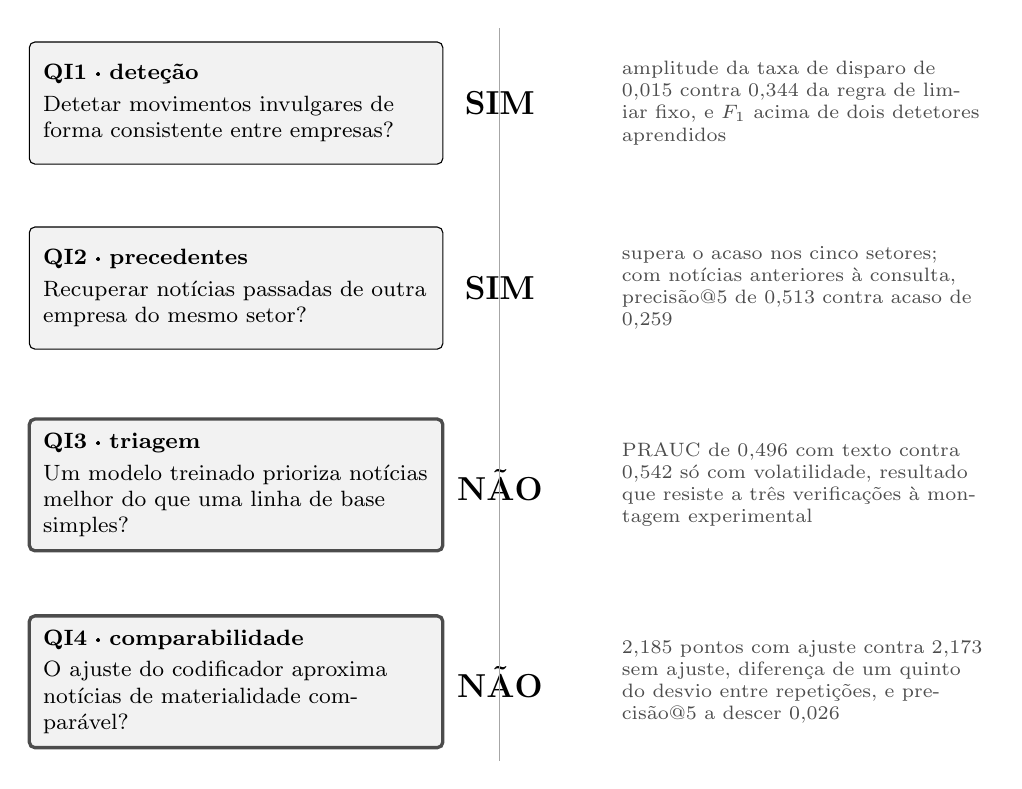
\begin{tikzpicture}[font=\footnotesize,
  cx/.style={draw, rounded corners=2pt, align=left, inner sep=5pt, text width=4.9cm,
             minimum height=1.55cm, fill=black!5},
  neg/.style={cx, draw=black!70, very thick},
  ver/.style={font=\bfseries\large, align=center},
  num/.style={align=left, text width=4.6cm, font=\scriptsize, text=black!70},
]
  \node[cx] (q1) at (0,0) {\textbf{\gls{QI}1 · deteção}\\[2pt]
    Detetar movimentos invulgares de forma consistente entre empresas?};
  \node[ver] at (3.35,0) {SIM};
  \node[num] at (7.2,0) {amplitude da taxa de disparo de $0{,}015$ contra $0{,}344$ da regra
    de limiar fixo, e $F_1$ acima de dois detetores aprendidos};

  \node[cx] (q2) at (0,-2.35) {\textbf{\gls{QI}2 · precedentes}\\[2pt]
    Recuperar notícias passadas de outra empresa do mesmo setor?};
  \node[ver] at (3.35,-2.35) {SIM};
  \node[num] at (7.2,-2.35) {supera o acaso nos cinco setores; com notícias anteriores à
    consulta, precisão@5 de $0{,}513$ contra acaso de $0{,}259$};

  \node[neg] (q3) at (0,-4.85) {\textbf{\gls{QI}3 · triagem}\\[2pt]
    Um modelo treinado prioriza notícias melhor do que uma linha de base simples?};
  \node[ver] at (3.35,-4.85) {NÃO};
  \node[num] at (7.2,-4.85) {\gls{PRAUC} de $0{,}496$ com texto contra $0{,}542$ só com
    volatilidade, resultado que resiste a três verificações à montagem experimental};

  \node[neg] (q4) at (0,-7.35) {\textbf{\gls{QI}4 · comparabilidade}\\[2pt]
    O ajuste do codificador aproxima notícias de materialidade comparável?};
  \node[ver] at (3.35,-7.35) {NÃO};
  \node[num] at (7.2,-7.35) {$2{,}185$ pontos com ajuste contra $2{,}173$ sem ajuste, diferença de um quinto do desvio entre repetições, e precisão@5 a descer $0{,}026$};

  \draw[black!35] (3.35,-8.35) -- (3.35,0.95);
\end{tikzpicture}
\caption[As quatro questões de investigação e as respostas obtidas]{As quatro respostas, com as duas
respostas negativas apresentadas com o mesmo destaque das duas afirmativas. A resposta à segunda questão
limita-se às alternativas avaliadas e ao critério aproximado de relevância setorial.}
\label{fig:con_scorecard}
\end{figure}

\begin{figure}[ht]
\centering
\begin{tikzpicture}[font=\scriptsize,
  cx/.style={draw=black!55, rounded corners=1.5pt, fill=black!4, align=center,
        text width=2.7cm, minimum height=1.42cm, inner sep=2pt},
  res/.style={cx, fill=black!10, draw=black!75, line width=0.8pt},
  qi/.style={font=\bfseries\footnotesize, align=center},
  cab/.style={font=\scriptsize\itshape, text=black!60, align=center},
  nao/.style={font=\scriptsize, text=black!58, align=left, text width=13.7cm},
  seta/.style={-{Stealth[length=3.5pt]}, draw=black!45},
]
  \node[cab] at (1.5,1.16) {a pergunta};
  \node[cab] at (4.6,1.16) {como se mede};
  \node[cab] at (7.7,1.16) {contra o quê};
  \node[cab] at (10.8,1.16) {o resultado};
  \node[qi] at (-0.72,0.0) {QI1};
  \node[cx] (c00) at (1.5,0.0) {movimentos invulgares, entre empresas?};
  \node[cx] (c01) at (4.6,0.0) {amplitude da taxa de disparo, sem rótulos};
  \node[cx] (c02) at (7.7,0.0) {limiar fixo de três por cento};
  \node[res] (c03) at (10.8,0.0) {$0{,}015$\\ contra $0{,}344$};
  \draw[seta] (c00) -- (c01);
  \draw[seta] (c01) -- (c02);
  \draw[seta] (c02) -- (c03);
  \node[nao, anchor=west] at (-0.35,-1.06) {o que daqui não decorre: não que a parametrização escolhida seja a melhor da família};
  \node[qi] at (-0.72,-2.72) {QI2};
  \node[cx] (c10) at (1.5,-2.72) {precedentes de outra empresa do setor?};
  \node[cx] (c11) at (4.6,-2.72) {precisão@5, rótulo aproximado pelo setor};
  \node[cx] (c12) at (7.7,-2.72) {acaso, sobreposição de palavras, recência};
  \node[res] (c13) at (10.8,-2.72) {$0{,}395$\\ contra $0{,}117$};
  \draw[seta] (c10) -- (c11);
  \draw[seta] (c11) -- (c12);
  \draw[seta] (c12) -- (c13);
  \node[nao, anchor=west] at (-0.35,-3.78) {o que daqui não decorre: não mede vantagem sobre um filtro pelo setor da consulta};
  \node[qi] at (-0.72,-5.44) {QI3};
  \node[cx] (c20) at (1.5,-5.44) {triagem melhor que a volatilidade?};
  \node[cx] (c21) at (4.6,-5.44) {PR-AUC no bloco de teste reservado};
  \node[cx] (c22) at (7.7,-5.44) {volatilidade dos vinte dias anteriores};
  \node[res] (c23) at (10.8,-5.44) {$0{,}496$\\ contra $0{,}542$};
  \draw[seta] (c20) -- (c21);
  \draw[seta] (c21) -- (c22);
  \draw[seta] (c22) -- (c23);
  \node[nao, anchor=west] at (-0.35,-6.5) {o que daqui não decorre: não que o texto de notícias seja inútil para a tarefa};
\end{tikzpicture}
\caption[O percurso de cada questão até à resposta]{Para cada questão, o percurso da pergunta até ao resultado, e a linha que delimita o alcance desse resultado. As três primeiras colunas são o protocolo, fixado antes da medição; a quarta é o valor obtido contra a alternativa. A linha inferior de cada bloco é a que distingue uma avaliação de uma demonstração, e é desenvolvida nas subsecções que se seguem.}
\label{fig:con_cadeia}
\end{figure}

\subsection{Deteção de movimentos invulgares}

A resposta à \gls{QI}1 é afirmativa. Um \emph{z}-score sobre uma janela deslizante de vinte dias assinala dias raros a uma taxa
praticamente idêntica em empresas de volatilidades muito distintas. A amplitude entre a empresa
mais e a menos assinalada é de $0{,}015$, contra $0{,}344$ de uma regra de limiar fixo em três por
cento. Contra um rótulo aproximado, o método obtém
$F_1 = 0{,}516$ e a regra fixa $0{,}218$. Sujeito a um protocolo causal equivalente, o mesmo método
supera ainda dois detetores concebidos para esta tarefa, com $F_1$ de $0{,}530$ contra $0{,}269$ do
\emph{Isolation Forest} \autocite{liu2008isolation} e $0{,}280$ do \emph{Local Outlier Factor}
\autocite{breunig2000lof}.

A configuração implantada não é, porém, a melhor medida dentro da própria família. Com a mesma
cobertura, um estimador com decaimento exponencial obtém $F_1 = 0{,}664$ e uma janela de sessenta
dias obtém $0{,}678$, contra os $0{,}516$ da configuração em produção. O que a \gls{QI}1 estabelece
é que a família deslizante supera o limiar fixo e os dois detetores aprendidos, e não que a
parametrização escolhida seja a melhor dessa família.

Este resultado é menos surpreendente do que a diferença de valores sugere, e a literatura permite
situá-lo. Os dois detetores aprendidos definem raridade a partir da geometria dos dados, um por
isolamento do ponto e outro por comparação de densidades, e foram concebidos para espaços com
múltiplas variáveis em interação. O problema tratado apresenta uma única série de retornos por empresa, na qual a estrutura
relevante é temporal e não geométrica: períodos de agitação sucedem-se a períodos calmos. É a
propriedade que os modelos \gls{ARCH} e \gls{GARCH} formalizam \autocite{engle1982arch,
bollerslev1986garch}. A janela deslizante capta-a diretamente; um detetor treinado sobre o
conjunto completo teria de a aprender. Quando a suposição embutida
num método simples coincide com a estrutura efetiva do problema, a margem para a superar é reduzida.

O alcance da resposta é delimitado por três condições. A comparação incide sobre quinze empresas de
grande capitalização, selecionadas em 2026 e avaliadas sobre o passado, que sobreviveram por
construção; sobre três anos de cotações e sobre um único mercado. O rótulo utilizado como argumento
secundário é ele próprio relativo à volatilidade de cada empresa, razão pela qual o argumento
principal é a consistência da taxa de disparo, que não depende de rótulos. O limiar de três por cento
da regra alternativa não foi otimizado, pelo que o que a comparação estabelece não é que nenhum
limiar fixo obtivesse melhor resultado, mas que uma regra de limiar fixo mede uma quantidade distinta
da pretendida.

\subsection{Recuperação de precedentes}
\label{sec:con_qi2}

A resposta à \gls{QI}2 é afirmativa face às alternativas avaliadas. Sobre o corpus
recente, a recuperação por semelhança de frase \autocite{reimers2019sbert} obtém precisão@5 de
$0{,}395$, contra $0{,}196$ da sobreposição de vocabulário, $0{,}117$ da escolha aleatória e
$0{,}204$ da apresentação das notícias mais recentes. Também aqui o modelo implantado não é o melhor
medido: uma variante de maior dimensão obtém $0{,}422$ sobre o mesmo protocolo, e foi preterida por
custo computacional.

O valor agregado não constitui, porém, a forma adequada de enunciar o resultado. Oitenta e quatro por cento das
notícias do corpus pertence ao setor da tecnologia, o que torna disponível uma estratégia que
dispensa qualquer modelo e sequer observa a consulta, consistindo em devolver invariavelmente
notícias desse setor; a sua precisão iguala a fração de consultas de tecnologia, $0{,}840$ no corpus completo. Essa
estratégia é inútil enquanto produto, dado que acerta em todas as consultas de um setor e em nenhuma
dos quatro restantes, mas a sua existência demonstra que o agregado mede em parte a composição do
corpus.

A comparação que controla esta composição realiza-se dentro de cada setor, onde o método supera o
respetivo valor de referência nos cinco. A margem absoluta é maior no setor mais abundante, com
$+0{,}220$ na tecnologia; nos setores escassos, onde o valor de referência ronda $0{,}100$, o método
obtém várias vezes esse valor com margem absoluta menor. O alcance é o das alternativas avaliadas:
se a seleção pudesse usar o setor conhecido da consulta, bastaria filtrar por esse setor para
satisfazer o rótulo, desde que existissem candidatos suficientes. A análise por setor não mede
vantagem semântica sobre esse filtro.

Duas verificações adicionais delimitam a resposta. Sobre o corpus histórico completo, com aproximadamente oitenta mil notícias de seis anos, a
precisão sobe para $0{,}595$. O valor de referência sobe também, e mais depressa, pelo que a
margem desce de $+0{,}278$ para $+0{,}262$.
O método não se degrada com a escala, nem melhora com ela. Exigir que o precedente seja anterior
à consulta reduz a precisão
para $0{,}513$ e o valor de referência para $0{,}259$, com a margem a variar $0{,}008$. O método
conserva a vantagem sob esta restrição de anterioridade. O teste não impõe a maturação de oito
dias usada em produção e, por isso, não valida integralmente a disponibilidade dos desfechos.

A segunda ressalva tem consequências diretas sobre o produto. A recuperação identifica tema e não
direção: a concordância entre o sentido do movimento da notícia de consulta e o dos precedentes
situa-se em $0{,}708$ contra um valor de acaso de $0{,}688$, uma diferença de $0{,}020$. Duas
notícias podem tratar do mesmo assunto e o preço evoluir em sentidos opostos. O resultado é
coerente com o que a forma semiforte da hipótese dos mercados eficientes conduziria a esperar
\autocite{fama1970efficient}, segundo a qual a informação pública se encontra já refletida no preço,
sem que o trabalho a teste ou nela se apoie para estabelecer qualquer conclusão. A consequência
prática é apresentar os precedentes individualmente, com data e desfecho. O alerta histórico
reproduzido na Figura~\ref{fig:sis_alerta} inclui também uma média, que resume aqueles casos e
não constitui previsão para a notícia recebida.

Uma delimitação final respeita ao rótulo. A pertença ao mesmo setor aproxima a relevância de forma
verificável, sem coincidir com a propriedade que se pretendia medir. A linha de base lexical é a forma mais elementar da sua família, sem ponderação pela raridade dos
termos nem normalização pelo comprimento. Os dezassete pontos percentuais de vantagem medem a
distância a um ponto de partida, e não a uma função de ordenação afinada
\autocite{robertson2009bm25}.

\subsection{Triagem de notícias}

A resposta à \gls{QI}3 é negativa. Nenhuma variante que incorpora o texto do título supera uma linha
de base construída apenas com a volatilidade dos vinte dias anteriores, com $0{,}496$ de \gls{PRAUC}
contra $0{,}542$, e o índice de Brier acompanha a mesma ordenação. O resultado resiste a três verificações. A primeira repete a comparação concedendo ao texto as
melhores condições disponíveis, e eleva o seu melhor valor para $0{,}533$, sem alcançar a linha de
base. A segunda reamostra por grupos constituídos pela empresa e pelo dia, e mantém o intervalo a
excluir zero. A terceira repete a medição para nove combinações alternativas de limiar e horizonte
do rótulo, e a volatilidade iguala ou supera o modelo com texto nas nove.

A resposta ganhou precisão no decurso do trabalho e essa precisão altera o que dela se retira. As
comparações anteriores colocam as representações lado a lado e respondem, por conseguinte, à pergunta
sobre qual delas é melhor. A pergunta com maior utilidade para quem constrói um sistema é distinta e
consiste em determinar se o texto acrescenta ao que já é conhecido. Medida sobre a tabela de consulta
por empresa, que contém tudo o que o modelo conhece da empresa e nada da notícia, a resposta é
afirmativa: o título acrescenta $+0{,}012$ de \gls{PRAUC}, com intervalo entre $+0{,}004$ e
$+0{,}020$, que exclui zero. É a única ocasião em que uma representação de texto apresenta um
acréscimo detetável nesta tarefa.

O valor situa-se abaixo do limite de $0{,}02$ que o Capítulo~\ref{cap:avaliacao} fixou antes das
medições. O acréscimo observado fica abaixo desse critério prático; não estabelece um limite
garantido para o efeito do texto.

Três medições impedem que este acréscimo reabra o veredicto. A soma não supera a volatilidade isolada, e o intervalo da diferença contém zero. O acréscimo não
sobrevive à métrica que descreve o produto: a precisão dentro do orçamento de cinco alertas por
dia permanece em $0{,}662$ com e sem texto. A ordenação dentro de cada empresa mantém-se ao
nível do acaso. Estas medições não demonstram ganho operacional do texto: o rótulo é comum a
todas as notícias de uma empresa no mesmo dia, pelo que a métrica avalia a seleção de dias de
empresa e não a distinção entre títulos desse dia.

Existe uma linha de investigação estabelecida que utiliza texto para antecipar movimentos de preço
\autocite{xing2018nlffsurvey, ding2015deep}, e este resultado não a contradiz. A diferença não reside na dimensão do texto, uma vez que \textcite{ding2015deep} operam igualmente
sobre títulos, mas no tratamento que lhe é dado. Aqueles autores extraem estruturas de
acontecimento e treinam uma rede para prever a direção do movimento. Aqui os títulos são
comparados por semelhança, e a direção nunca é objeto de previsão. Os corpora e os horizontes de avaliação diferem igualmente. A
afirmação que este trabalho sustenta é mais estreita do que uma refutação: sob esta restrição de
dados e com esta família de métodos, o sinal textual nada acrescenta ao que a volatilidade recente
já indicava. O alcance do resultado limita-se, por isso, a um regime de recursos e a uma escolha de
representação, e não se estende à linguagem.

Existe, ainda assim, uma leitura teórica que o enquadra e que se enuncia com a mesma cautela. A
forma semiforte da hipótese dos mercados eficientes \autocite{fama1970efficient} sustenta que a
informação publicamente disponível se encontra já refletida no preço. Se assim for, um título
público não tem, no momento em que é lido, informação que os preços recentes não contenham, e o
resultado obtido é o que essa hipótese conduziria a esperar. A condição de recursos deste trabalho
agrava a expectativa em vez de a atenuar: entre a publicação de uma notícia e a sua deteção por
fontes gratuitas decorrem $353$ minutos de mediana, intervalo durante o qual qualquer reação do
mercado já ocorreu. O sistema observa, por construção, informação que deixou de ser nova.

Esta leitura é um enquadramento, sem estatuto de conclusão. O trabalho não testa a hipótese dos mercados
eficientes, e um resultado negativo obtido com uma família de métodos sobre um corpus concreto não
a confirma; confirmá-la exigiria um desenho que este não tem. O que a leitura acrescenta é a razão
pela qual o resultado é menos surpreendente do que a hipótese inicial supunha, e por que motivo a
sua correção mais provável não está na representação do texto mas no atraso com que ele chega.

\subsection{Comparabilidade de materialidade}
\label{sec:con_qi4}

A resposta é \textbf{não}, e é negativa nas duas metades da pergunta. O ajuste contrastivo do
codificador não melhora a comparabilidade de materialidade dos precedentes recuperados: o braço
treinado sobre a magnitude obtém $2{,}185$ pontos percentuais contra $2{,}173$ do modelo sem
ajuste, ou seja um valor pior, e o treinado sobre a direção obtém $2{,}157$. As duas diferenças
são cerca de um quinto do desvio entre repetições do próprio braço. E o ajuste tem um custo que a
medição separa: a precisão@5 por setor desce cerca de $0{,}026$ nos dois braços, com o mesmo
sinal e acima da dispersão.

O que distingue este resultado de uma montagem que falhou é o diagnóstico que o precede. A
primeira tentativa colapsou o codificador, e foi descartada sem que as suas métricas fossem
lidas; os dois braços que produziram os valores acima deslocaram substancialmente o espaço face
ao modelo de partida e preservaram a geometria das semelhanças. Treinaram, portanto, e o que não
se confirma é a hipótese.

A comparação entre os dois braços era a parte da experiência destinada a separar magnitude de
direção, e não encontrou a assimetria que a motivou: os dois são praticamente indistinguíveis
entre si, tanto no diagnóstico como nas duas medidas. A conjetura de que a magnitude seria
parcialmente aprendível do texto onde a direção não o é permanece, por conseguinte, sem apoio
nesta montagem.

Um terceiro braço, partindo de um codificador de domínio, foi treinado como controlo e
colapsou, pelo que as suas métricas também não foram lidas. O diagnóstico mostra a razão: o
espaço desse codificador é, antes de qualquer ajuste, muito menos disperso do que o do
codificador de frases, e a taxa que este tolera basta para o fazer degenerar. O limiar de
colapso é uma propriedade do modelo de partida e não da receita.

A consequência para o sistema é a de manter o que já fazia. A base de casos organiza-se por tema,
e o alerta declara que a semelhança é de tema; este resultado estabelece que, por esta via, não é
possível acrescentar-lhe a garantia de que a magnitude do precedente é comparável. Fica assim
reforçada a decisão descrita na Secção~\ref{sec:con_qi2} de apresentar os casos um a um em vez de
os resumir por uma média.

\section{Objetivos alcançados}
\label{sec:con_objetivos}

Dos quatro objetivos enunciados na Secção~\ref{sec:intro_objetivos}, três encontram-se integralmente
cumpridos e um cumprido com a ressalva descrita adiante.

O primeiro objetivo, construir o sistema completo desde a aquisição de dados até à entrega do alerta,
está cumprido. Os dois gatilhos funcionam de ponta a ponta em produção, sobre fontes gratuitas, e o
percurso de um acontecimento está documentado no Capítulo~\ref{cap:sistema} com os valores de um caso
real.

O segundo objetivo, avaliar os componentes com linhas de base transparentes, está cumprido
para as três técnicas em que existe um referente externo. Num dos casos foi além do previsto: o
detetor foi comparado não apenas com uma regra de limiar fixo, mas também com dois métodos
aprendidos.
A decomposição do movimento constitui a ressalva: não existe verdade de terreno contra a qual medir a
exatidão de uma repartição, pelo que se mediu o que nela permanece falsificável, correspondente à
qualidade do ajuste e à capacidade de discriminar. Ficaram por realizar comparações internas que
seriam possíveis, como a do modelo de um fator contra o de dois fatores ou a das sensibilidades
brutas contra as encolhidas.

O terceiro objetivo, garantir que as explicações apresentadas são fiéis ao que o sistema calculou,
está cumprido por construção, sem depender de verificação posterior. Cada valor exibido provém do objeto que
o calculou, e o texto é composto a partir dessas peças, pelo que não é possível ao alerta enunciar um
valor distinto do que o sistema obteve. A fidelidade é, contudo, uma propriedade do sistema, e não da
relação entre o sistema e quem o lê; a utilidade das explicações para um investidor particular não
foi medida, e a Secção~\ref{sec:con_limitacoes} trata essa ausência.

O quarto objetivo, reportar os resultados obtidos incluindo os que não confirmem as expectativas
iniciais, está cumprido. A resposta negativa à \gls{QI}3 aparece na Figura~\ref{fig:con_scorecard}
e no corpo deste capítulo com o mesmo destaque das restantes, acompanhada das três verificações a
que foi submetida e das três ocasiões em que uma técnica mais simples superou uma mais
sofisticada.

\section{Limitações}
\label{sec:con_limitacoes}

Esta secção enumera as limitações do trabalho por ordem de importância. A
Tabela~\ref{tab:con_limites} apresenta-as em conjunto, com o trabalho que encerraria cada uma e a
natureza do respetivo custo; o texto que se segue desenvolve as quatro de maior consequência e
resume as restantes. A maioria está quantificada. Duas não o estão por natureza: a ausência de
estudo controlado é uma ausência e não uma medida, e a distância entre cada rótulo e a
propriedade que aproxima só seria mensurável contra uma anotação humana que não existe.

\begin{table}[!htbp]
\caption[As limitações e o trabalho que as encerraria]{As onze limitações, por ordem de
importância, com o trabalho que encerraria cada uma e a natureza do custo desse trabalho. As duas
que dependem de tempo de calendário são as que exigem julgamento humano, e são também as duas de
que as restantes mais dependem: enquanto não existir uma amostra anotada por pessoas, nem a
utilidade das explicações nem a qualidade dos rótulos deixam de ser aproximações.}
\label{tab:con_limites}
\centering
\footnotesize
\begin{tabular}{@{}L{0.33\textwidth} L{0.32\textwidth} L{0.20\textwidth}@{}}
\toprule
\tabhead{Limitação} & \tabhead{O que a encerra} & \tabhead{Custo} \\
\midrule
Nenhum estudo controlado com pessoas & Executar o protocolo desenhado, com seis a dez participantes &
tempo de calendário \\
A pontuação é quase constante dentro de cada empresa & Entradas que variem de um título para o
seguinte & reduzido; re-treina \\
O rótulo pode favorecer a linha de base vencedora & Reconstruir o alvo com sensibilidades
estimadas & reduzido; re-treina \\
Os rótulos são aproximações verificáveis & Anotar uma amostra com julgamento humano &
tempo de calendário \\
O alerta afirma mais evidência do que a que possui & Medir o impacto por notícia e não por dia &
dados intradiários \\
A composição por empresa varia entre os três blocos & Uma divisão de composição constante & reduzido; reavalia \\
Apenas o título é lido, e não o corpo do artigo & Recolher e representar o texto integral &
dados novos \\
A repartição nem sempre está bem estimada & Comparar um fator com dois; o ajuste já é exibido & reduzido; reavalia \\
A deriva é medida e não corrigida & Re-treinar com o registo de produção & reduzido; re-treina \\
A cobertura das fontes é incompleta e desigual & Acrescentar fontes, ou declarar o limite &
fora de controlo \\
As três causas do atraso não estão separadas & Registar quando cada item surge no fluxo &
instrumentação \\
\bottomrule
\end{tabular}
\end{table}

\paragraph{Não foi realizado um estudo controlado com utilizadores.}
Esta é a lacuna de maior peso. O sistema assenta na hipótese de que uma explicação acompanhada
da respetiva evidência conduz um não especialista a uma decisão melhor, e essa hipótese não foi
submetida a um desenho experimental. O protocolo existe, com participantes, tarefas e critérios
definidos, e não foi executado. O que existe, e está reportado na
Secção~\ref{sec:av_feedback}, é retorno recolhido em contexto real: leitores do canal público
classificam os alertas que recebem, sob regras de análise fixadas antes do primeiro voto, e a
recolha prossegue. A literatura é explícita quanto ao peso desta ausência: afirmações
de interpretabilidade exigem avaliação e não se estabelecem por declaração
\autocite{doshivelez2018considerations}. A razão não é formal. O efeito de uma explicação sobre uma pessoa
não é dedutível da sua construção: sabe-se que a confiança em sistemas automáticos falha nos dois
sentidos, com o utilizador a ignorar um aviso correto ou a aceitar um aviso incorreto
\autocite{lee2004trust}, e que a mera presença de uma explicação aumenta a aceitação de respostas
erradas \autocite{bansal2021whole}. O sistema foi construído para produzir confiança apropriada,
apresentando evidência em vez de emitir um veredicto, mas que o consiga permanece uma hipótese. Na
ausência do estudo, os dois modos de falha são indistinguíveis nos registos: um alerta ignorado e um
alerta indevidamente acreditado produzem a mesma ausência de dados.

A distinção entre as duas coisas determina o que cada uma permite afirmar. O retorno do
canal é observacional: vota quem quer, o que desloca a amostra para os extremos; nenhum
grupo recebeu a variação de preço sem a explicação que a acompanha, pelo que nada atribui a
utilidade à explicação em si; e o canal é público, pelo que se desconhece se quem responde
pertence ao público que este trabalho assume. O que esses votos medem é utilidade percebida
por quem se dispôs a responder. A hipótese fundadora diz respeito a decisão melhor, que é
outra quantidade, e é essa que permanece por testar.

Duas observações da literatura alteram o peso desta ausência, em sentidos opostos, e ambas devem
constar. A primeira agrava-o. A hipótese fundadora não é apenas indemonstrada neste trabalho: tem
contra si medições publicadas. \textcite{waa2021xai} não encontraram diferença entre a explicação
por exemplos e a ausência de explicação, e \textcite{cau2023logicstyle} encontraram, numa tarefa de
negociação de ações com não-especialistas, desempenho inferior do estilo indutivo face aos estilos
abdutivo e dedutivo quando o modelo está confiante. Enquanto o estudo não se fizer, a posição
honesta não é «por demonstrar», é «por demonstrar, e com evidência publicada a apontar em sentido
contrário». A Secção~\ref{sec:ctx_xai} enuncia a razão pela qual este trabalho pode ainda assim
esperar desfecho diferente, uma vez que entrega o cálculo subjacente e é a falta dele que aqueles
autores responsabilizam pelo resultado; mas uma expectativa fundamentada continua a ser uma expectativa.

A segunda situa-o. O trabalho publicado mais próximo desta classe de sistema
\autocite{muntermann2009ubiquitous} avaliou o artefacto por simulação e remeteu igualmente o
estudo com utilizadores para investigação futura, quinze anos antes deste. Na revisão que sustenta
o Capítulo~\ref{cap:contexto} não se encontrou, nesta classe de sistema, nenhum estudo que
estabeleça por via causal que alertas acompanhados de evidência melhoram a decisão de um não
especialista. Isto não desculpa a ausência nem a torna menos limitação, mas altera o que ela
significa: não é uma etapa que este trabalho tenha saltado, é uma etapa que a área ainda não deu.

\paragraph{O modelo implantado não podia executar a função que lhe foi atribuída.}
A variante colocada em produção como porta de decisão recebe sete entradas de nível de empresa, uma
de nível do dia e uma única que varia de um título para o seguinte, correspondente ao comprimento do
título. A sua pontuação é, por aritmética e não por acidente, quase constante dentro de cada
empresa: a amplitude média dentro de cada empresa é de $0{,}072$ e a amplitude entre as medianas das
empresas é de $0{,}392$. Em $48\%$ dos títulos distintos, o resultado estava determinado antes de o
título ser lido.

Duas afirmações têm de ser separadas, uma vez que apenas uma corresponde a erro. O resultado da
\gls{QI}3 mantém-se, porque a variante com texto dispunha de trezentos e oitenta e quatro números
por título e ainda assim perdeu. A decisão de produto estava errada, e a razão é de método: a
escolha foi tomada por uma métrica que interroga a ordenação do conjunto completo, quando o produto
necessitava de selecionar oportunidades sob um orçamento diário. O rótulo por empresa e dia
não permite avaliar a distinção entre dois títulos publicados nessa mesma unidade.

O sistema foi alterado e o modelo deixou de constituir porta para passar a critério de ordenação.
Essa alteração não está validada. Sobre as $825$ decisões maturadas em produção, agrupadas nas $239$
unidades independentes que o rótulo admite, a capacidade de ordenação é de $0{,}486$, com intervalo
entre $0{,}403$ e $0{,}571$, que contém o acaso. A ordenação é a utilização menos indefensável do
modelo, e não uma utilização demonstrada.

Esta falha pertence a uma classe descrita na literatura de sistemas de aprendizagem em produção.
\textcite{sculley2015debt} identificam um custo que não figura em nenhuma métrica de qualidade, e
que vem de dependências de dados e do emaranhamento entre componentes: a validade de uma peça
depende de suposições sobre outra que nunca foram enunciadas. O modelo foi avaliado isoladamente,
sobre a distribuição do conjunto de treino, e implantado atrás de dois filtros que a alteram. Nenhum
teste falhou e nenhum registo assinalou anomalia. Um componente aprendido é avaliado onde é treinado
e é útil onde é colocado, e quando esses dois lugares diferem a diferença não se anuncia.

\paragraph{O rótulo pode favorecer a linha de base vencedora.}
O rótulo desconta o movimento do mercado assumindo sensibilidade unitária, pelo que o seu erro não é
aleatório: é maior nas ações mais sensíveis ao mercado, que são tipicamente as mais voláteis. A
linha de base vencedora é exatamente a volatilidade. Com o que está medido não é possível separar a
hipótese de a volatilidade prever melhor a materialidade da hipótese de a volatilidade prever melhor
o erro do rótulo. Tanto o nível como a ordenação das métricas da \gls{QI}3 ficam por isso
condicionados ao rótulo utilizado.

\paragraph{O alerta afirma mais evidência do que a que possui.}
Quando exibe três precedentes concordantes quanto ao sentido do movimento, o alerta apresenta essa
concordância como resultante de três observações. O impacto é, porém, medido por par constituído
pela empresa e pelo dia, pelo que três títulos da mesma empresa no mesmo dia partilham o valor por
construção. Sobre os $247$ alertas com precedentes entregues, em $36{,}8\%$ os casos exibidos
assentam em menos dias distintos do que o número de casos apresentados, e em $11{,}3\%$
correspondem todos ao mesmo
dia; dos $120$ alertas que afirmam unanimidade, $23{,}3\%$ apoiam-se num único dia. A formulação do
texto foi corrigida para contar dias e não títulos, o que torna a afirmação verdadeira. A causa
subsiste: enquanto o impacto for medido por dia, duas notícias do mesmo dia não constituem duas
observações independentes.

\paragraph{As restantes sete, em síntese.}
Os \textbf{rótulos são aproximações}: relevância é aproximada pela pertença ao mesmo setor,
materialidade pela ocorrência de um movimento acima de um limiar, e raridade por um percentil dos
retornos da própria empresa. As três são objetivas e verificáveis, e nenhuma corresponde exatamente
à propriedade que se pretendia medir. A dependência de aproximações não é particularidade deste
trabalho: em domínios financeiros vizinhos, como a deteção de fraude, os métodos não supervisionados
ocupam posição central pela escassez de anomalias rotuladas \autocite{ahmed2016financial}.

A \textbf{composição por empresa varia entre os três blocos}. O treino contém treze empresas e
o teste nove: oito são comuns, cinco só aparecem no treino e uma só no teste. Esta última
representa $17{,}1\%$ das linhas de teste; as empresas conhecidas representam os restantes
$82{,}9\%$. Existe sobreposição substancial, mas as frequências mudam. A comparação não isola
o efeito dessa mudança do desempenho do modelo, nem demonstra generalização uniforme a empresas novas.

As \textbf{notícias são lidas apenas ao nível do título}. O sistema representa o título e não o
corpo do artigo, o que limita o que a representação de texto pode captar e constitui explicação
plausível, ainda que não confirmada, para o resultado negativo da \gls{QI}3. As revisões de análise
textual em finanças descrevem trabalhos que operam sobre documentos completos
\autocite{kearney2014textual}, e um título é a parte do documento onde mais informação foi
descartada.

A \textbf{repartição de um movimento nem sempre está bem estimada}. A soma das três parcelas
verifica-se por construção e não valida coisa alguma. A medida informativa é o coeficiente de
determinação na janela de estimação, cuja mediana foi de $0{,}460$ e que numa das dezassete empresas
assumiu valor negativo, o que significa que naquela janela o ajuste não descrevia os dados.
A interface passou a exibir esse coeficiente ao lado das três parcelas, comparado com a mediana
da lista vigiada, e a nomear em palavras o caso em que o ajuste não descreve os dados. A estimativa
não melhora por ser exibida, e a limitação subsiste; o que deixa de suceder é o leitor receber
uma repartição sem meio de saber quando ela é fraca. O encolhimento ponderado pela precisão \autocite{vasicek1973beta} limita o dano de uma
estimativa má sem a transformar numa estimativa boa.

A \textbf{deriva é medida e não corrigida}. Os parâmetros foram estimados entre 2018 e 2023 e não
voltaram a ser ajustados. Entre o bloco de treino e o de teste, o índice de estabilidade
populacional situa a volatilidade dos vinte dias na banda de deslocamento significativo, com
$0{,}281$, que é a entrada de que o modelo mais depende. A literatura de deriva de conceito trata
deste problema, com uma taxonomia da mudança e estratégias de deteção e adaptação
\autocite{gama2014survey}; aqui existe a deteção, sem a adaptação. A arquitetura que a forneceria
está definida na Secção~\ref{sec:sis_ciclo}, com gatilho condicional, janela deslizante e porta de
promoção, e não foi executada: a limitação é de execução e não de desenho.

A \textbf{cobertura das fontes é incompleta e desigual}. Existia pelo menos uma notícia relevante em
$88{,}5\%$ dos $417$ dias considerados invulgares pelo detetor, e a empresa pior coberta situa-se
nos $50\%$. Nos dias restantes nenhuma alteração ao sistema produz efeito, uma vez que uma notícia
não associada à empresa pela fonte não chega a entrar no percurso. O valor é um limite superior:
estabelece que existia uma notícia, e não que tenha chegado a notícia adequada.

O \textbf{atraso está na descoberta, e as suas três causas não estão separadas}. Sobre os $278$ alertas
com hora de publicação e de envio, a mediana entre a publicação e a deteção é de $353$ minutos, e a
mediana entre a deteção e a entrega é de $5$ segundos. A passagem de um agendador de melhor esforço
para um ciclo de sessenta segundos não reduziu o atraso, o que exclui a cadência de consulta como
explicação. Restam três causas que o histórico não separa, e apenas uma delas, a de a fonte listar
tarde, seria atenuada por um serviço pago; as outras duas subsistem com qualquer fonte.

\section{Trabalho futuro}
\label{sec:con_futuro}

As linhas enunciadas nesta secção derivam das limitações da secção anterior, segundo a
correspondência apresentada na Tabela~\ref{tab:con_limites}, e estão ordenadas pela relação entre o
efeito esperado e o custo. Uma lista de trabalho futuro que não derive de limitações medidas
constitui uma justificação sob outra forma. A Figura~\ref{fig:con_futuro} agrupa-as pelo que
cada uma exige antes de poder ser executada.

\begin{enumerate}
  \item \textbf{Executar o estudo com utilizadores.} Seis a dez participantes, com sessões de
        aproximadamente quinze minutos, comparando a leitura de um facto isolado com a leitura do
        alerta completo. Encerra a afirmação central do trabalho, que é a de que a evidência
        apresentada junto do alerta conduz a uma decisão melhor. Partilha com a construção de um
        alvo anotado, terceiro item desta lista, a propriedade de nenhum meio computacional o
        acelerar, uma vez que ambos dependem de julgamento humano. Outras afirmações permanecem
        por verificar independentemente dele, entre as quais a qualidade dos três rótulos, a
        utilidade do modelo sobre a população que efetivamente observa e a estabilidade do
        resultado entre períodos.
  \item \textbf{Dotar o modelo de decisão de entradas que variem com a notícia.} É a correção direta
        da limitação de maior consequência técnica, e o seu custo é reduzido, dado que as duas
        quantidades mais evidentes já são calculadas pelo sistema: a semelhança do melhor precedente
        recuperado e a concordância de direção entre os precedentes. Ao contrário da volatilidade e
        do setor, ambas variam de um título para o seguinte.

  \item \textbf{Construir um alvo com julgamento humano.} A anotação de uma amostra de dias,
        identificando quais das notícias hoje suprimidas deveriam passar e quais das que passam nada
        acrescentam, forneceria pela primeira vez um alvo real para otimizar, em substituição do
        ajuste de constantes contra uma aproximação. A mesma amostra permitiria estimar a qualidade
        dos três rótulos utilizados.

  \item \textbf{Reconstruir o rótulo com sensibilidades estimadas.} O rótulo da triagem desconta o
        movimento do mercado assumindo sensibilidade unitária, o que introduz um erro correlacionado
        com a volatilidade da empresa, que é precisamente a linha de base vencedora. Refazer o alvo
        com as sensibilidades encolhidas descritas na Secção~\ref{sec:met_decomposicao} e repetir as
        seis famílias de modelos determinaria se a ordenação obtida resiste a uma definição
        alternativa de materialidade.

  \item \textbf{Ler o corpo dos artigos e não apenas o título.} É a hipótese mais direta para
        explicar o resultado negativo da \gls{QI}3 e é verificável com o protocolo já construído,
        exigindo apenas a recolha do texto integral.

  \item \textbf{Detetar histórias repetidas por significado.} A supressão de repetições assenta hoje
        em sobreposição de vocabulário, e a sua realização por semelhança utilizaria a técnica de que
        o sistema já dispõe. O ponto é mais relevante do que a sua dimensão técnica sugere: se o
        investidor particular adquire os ativos que lhe captam a atenção
        \autocite{barber2008glitters}, um sistema que comunica a mesma história três vezes não está a
        informar, mas a amplificar o mesmo estímulo.

  \item \textbf{Eliminar a assimetria de referencial do retorno do próprio dia.} A entrada
        corresponde, no treino, ao movimento completo do dia da notícia, e em produção à última
        barra disponível no momento da pontuação. Substituí-la pelo retorno acumulado até à
        publicação, ou, de forma mais conservadora, pelo retorno da véspera, elimina a diferença e
        permite reportar o desempenho sob um referencial único. O efeito na comparação entre
        modelos permanece por medir: exige reconstruir as entradas e repetir o treino e a avaliação.

  \item \textbf{Agrupar os precedentes por par de empresa e dia antes da seleção.} A correção
        aplicada ao texto do alerta tornou a afirmação verdadeira sem remover a causa. Selecionar os
        candidatos depois de agrupar por dia, exibindo de cada dia apenas o título mais próximo,
        elimina na origem a possibilidade de um dia observado três vezes ser apresentado como três
        casos concordantes.

  \item \textbf{Expor a qualidade do ajuste na própria mensagem.} A repartição de um movimento é
        exibida com a mesma confiança quando o coeficiente de determinação da janela é elevado e
        quando é negativo. Apresentá-lo junto da repartição, e acrescentar uma nota explícita abaixo
        de um limiar mínimo, converte uma limitação hoje declarada apenas no documento numa
        propriedade observável por quem lê o alerta.

  \item \textbf{Re-treinar o modelo com o registo de produção.} A deriva está medida e os rótulos
        novos derivam dos preços, pelo que a execução é possível. O impedimento não é técnico, uma
        vez que um re-treino alteraria os valores reportados neste documento e exigiria tempo de
        avaliação próprio.
\end{enumerate}

\begin{figure}[ht]
\centering
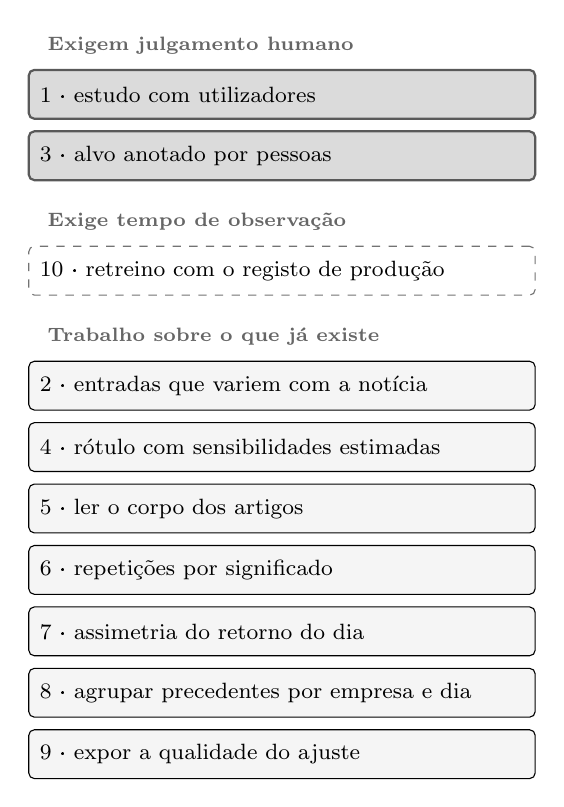
\begin{tikzpicture}[font=\footnotesize,
  it/.style={draw, rounded corners=2pt, align=left, inner sep=4pt, text width=6.15cm,
             minimum height=0.62cm, fill=black!4},
  hum/.style={it, fill=black!14, draw=black!65, thick},
  obs/.style={it, fill=white, draw=black!55, dashed},
  rot/.style={font=\scriptsize\bfseries, text=black!60, anchor=west},
]
  \node[rot] at (0,0.62) {Exigem julgamento humano};
  \node[hum] (a) at (3.1,0)     {1 · estudo com utilizadores};
  \node[hum] (b) at (3.1,-0.78) {3 · alvo anotado por pessoas};

  \node[rot] at (0,-1.62) {Exige tempo de observação};
  \node[obs] (c) at (3.1,-2.24) {10 · retreino com o registo de produção};

  \node[rot] at (0,-3.08) {Trabalho sobre o que já existe};
  \node[it] (d) at (3.1,-3.70) {2 · entradas que variem com a notícia};
  \node[it] (e) at (3.1,-4.48) {4 · rótulo com sensibilidades estimadas};
  \node[it] (f) at (3.1,-5.26) {5 · ler o corpo dos artigos};
  \node[it] (g) at (3.1,-6.04) {6 · repetições por significado};
  \node[it] (h) at (3.1,-6.82) {7 · assimetria do retorno do dia};
  \node[it] (i) at (3.1,-7.60) {8 · agrupar precedentes por empresa e dia};
  \node[it] (j) at (3.1,-8.38) {9 · expor a qualidade do ajuste};
\end{tikzpicture}
\caption[As linhas futuras, por aquilo que as desbloqueia]{As dez linhas de trabalho futuro,
agrupadas pelo que cada uma exige antes de poder ser executada. Sete operam sobre componentes que
o sistema já possui e dependem apenas de trabalho técnico. Uma aguarda tempo de observação, que
começou a decorrer em setembro de 2026. Duas exigem julgamento humano e são as únicas que nenhum
meio computacional acelera, o que as coloca no caminho crítico apesar de não serem as de maior
custo técnico. A numeração é a da lista desta secção, que está ordenada pela relação entre o
efeito esperado e o custo.}
\label{fig:con_futuro}
\end{figure}

Um caminho foi considerado e não seguido, e as razões ficam registadas por serem necessárias a quem
retome o trabalho. A predição conformal permite devolver conjuntos de respostas com uma garantia
livre de distribuição \autocite{vovk2005algorithmic, angelopoulos2023conformal}, o que se ajusta a
uma ferramenta que recusa afirmar mais do que aquilo que sabe. Duas razões afastaram-na. A primeira é
que a garantia é marginal, valendo em média sobre os casos e não caso a caso, que é precisamente a
leitura que um utilizador não especializado faria.

A segunda é mais determinante: a garantia exige
permutabilidade entre calibração e teste, e estes dados constituem uma série temporal, na qual os
títulos chegam por ordem. É a mesma suposição que este trabalho recusa ao dividir o conjunto por data
e com embargo. A aplicação do método sem tratamento desse ponto produziria intervalos com uma
garantia que os dados não sustentam, substituindo um valor honesto por um valor com aparência de
rigor.

Três direções técnicas ficam igualmente registadas, e são de outra natureza. Não derivam de
limitações medidas, pelo que não integram a lista anterior; decorrem de decisões de implementação
que a Secção~\ref{sec:ctx_texto} enuncia e que o trabalho não teve razão para revisitar.

A primeira é a reordenação por codificador cruzado. A recuperação compara cada par de frases
através de vetores calculados uma única vez, opção que a escala da base de casos impõe. Um
codificador que processe as duas frases em conjunto produz uma comparação mais fina e é
impraticável sobre dezenas de milhares de casos, mas praticável sobre os vinte primeiros
resultados de uma consulta. O protocolo de avaliação já construído mede exatamente essa lista.

A segunda é a aprendizagem de ordenação sob restrição de orçamento. O problema que o produto
resolve não é classificar cada notícia isoladamente, mas escolher cinco por dia, e a métrica
principal do Capítulo~\ref{cap:avaliacao} interroga a primeira formulação. Existe uma família de
métodos dedicada à segunda, e a diferença entre as duas está medida neste trabalho sem ser
nomeada: é a distância entre a PR-AUC sobre o conjunto completo e a precisão dentro do orçamento.
\textcite{feng2021hybrid} estudam a ordenação de notícias pela sua influência sobre um ativo,
combinando as perspetivas do ativo e do acontecimento. Esse trabalho oferece uma formulação a
explorar; o benefício sob o orçamento diário deste sistema continua por medir.

A terceira é a substituição da procura exaustiva por um índice aproximado
\autocite{johnson2021faiss}, referida na Secção~\ref{sec:ctx_texto} como caminho de
crescimento. Com a dimensão atual da base a procura exata é praticável e exata, pelo que a
substituição não se justifica hoje; justificar-se-ia a partir de uma ordem de grandeza acima.

\section{Considerações finais}
\label{sec:con_final}

O trabalho partiu de três perguntas que um investidor particular formula perante um movimento de
preço, e a que as ferramentas gratuitas não respondem. Se o movimento é invulgar. Se a origem é a
empresa ou o mercado. E se existem precedentes com desfecho conhecido. Construiu-se um
sistema que responde às três com evidência verificável e sem emitir previsões. Três técnicas foram
comparadas com alternativas mais simples; na decomposição mediu-se a qualidade do ajuste.

O resultado com maior valor informativo é negativo. A hipótese de que o texto das notícias transportaria informação ausente dos preços não foi
confirmada sobre este corpus. A sua investigação produziu um diagnóstico de alcance superior ao da
questão que a originou. O componente aprendido foi avaliado sobre uma distribuição e implantado
sobre outra, e a métrica pela qual foi selecionado formulava uma pergunta distinta da que o
produto necessitava. Nenhum
teste automático assinalou a discrepância, porque cada componente cumpria o seu contrato e o que
estava errado era uma suposição sobre a ligação entre eles.

A restrição fundadora do trabalho, segundo a qual o sistema não produz previsões de preço, revelou-se
a decisão de maior alcance. Determina o que pode ser afirmado: toda a afirmação do sistema é confirmável contra o registo no
momento em que é lida. Determina a forma da explicação, que permite inspecionar os casos individuais
e os seus desfechos. E determina o critério de avaliação, que incide sobre a capacidade de identificar o que é
invulgar e não sobre a de antecipar. Um sistema que apresente evidência em lugar de veredictos entrega menos do que um sistema
que anuncie direções, e entrega apenas o que consegue sustentar.

\begin{figure}[!htbp]
\centering
\begin{tikzpicture}[font=\footnotesize,
  est/.style={draw, rounded corners=2pt, align=left, inner sep=3pt, text width=5.1cm,
              minimum height=0.95cm, fill=black!6},
  abe/.style={draw, dashed, rounded corners=2pt, align=left, inner sep=3pt, text width=5.1cm,
              minimum height=0.95cm, fill=white, draw=black!65, thick},
  cab/.style={font=\scriptsize\bfseries, text=black!65},
  >={Stealth[length=2.2mm]},
]
  \node[cab] at (0,0.82) {O QUE FICA ESTABELECIDO};
  \node[est] (a) at (0,0.10)  {cada quantidade provém do componente que a calculou};
  \node[est] (b) at (0,-0.95) {é confrontável com o registo no momento em que é lida};
  \node[est] (c) at (0,-2.00) {a política que decide o silêncio está documentada e medida};

  \node[cab] at (6.9,0.82) {O QUE NÃO FICA};
  \node[abe] (d) at (6.9,-0.25) {que esta explicação conduza a uma
    \textbf{decisão melhor}};
  \node[align=left, text width=5.1cm, font=\scriptsize, text=black!62] (e) at (6.9,-1.75)
    {É a hipótese fundadora do trabalho. Permanece por testar, e o seu teste é a primeira
     linha do trabalho futuro.};
  \draw[->, black!50] (d) -- (e);
  \draw[black!25] (3.45,1.0) -- (3.45,-2.5);
\end{tikzpicture}
\caption[A fronteira daquilo que o trabalho estabelece]{O limite exato da afirmação. À esquerda,
as três propriedades que o sistema demonstra e que se verificam por inspeção do que ele produz. À
direita, a proposição que o trabalho não testou: que apresentar a evidência junto do alerta
conduza a uma decisão melhor. A separação não é uma reserva de cortesia, uma vez que a segunda é
a hipótese que motivou o trabalho, e distingui-la do que ficou demonstrado é o que impede que a
primeira seja lida como se a segunda estivesse provada.}
\label{fig:con_fronteira}
\end{figure}

A contribuição enuncia-se, por isso, no seu nível exato. O que este trabalho estabelece é que
o sistema está tecnicamente preparado para sustentar explicações assentes em evidência histórica
verificável: cada quantidade apresentada provém do componente que a calculou, é confrontável com o
registo no momento em que é lida, e a política que decide o silêncio está documentada e medida. O
que este trabalho não estabelece é que essa forma de explicação conduza o investidor particular a
uma decisão melhor. Essa é a hipótese fundadora, permanece por testar, e o seu teste é o primeiro
item da secção anterior. A Figura~\ref{fig:con_fronteira}
apresenta a separação.
